\documentclass{Mayth}
\begin{document}
\maketitle
\tableofcontents
\chapter{初高衔接}
\section{高中数学第一课}
\marginnote{2024-7-21}
\begin{center}
	原文来源:\citet{JiangGaoZhongShuXueDiYiKeDeJiaoXueGouXiang2016}
\end{center}

俗话说,好的开头是成功的一半.进入高中后,学生对每门课的第一节课都充满了期待.高中数学起始课应避免一上来就讲新课内容,可设计成“导游课”,像导游一样,每到一个景点时,先给游客对景点的特色、亮点、注意事项等作一个全貌的介绍.建议高中数学第一课可从两个方面进行构想:\textbf{一方面通过一些实例介绍高中数学之美妙,强调高中数学之重要,对初、高中数学特点进行比较;另一方面介绍高中数学的学习方法}.

\subsection{例说高中数学之美妙}
兴趣是最好的老师!要让学生喜欢数学,最有效的动力就是要激发学生学习数学的热情,让学生的内心能真正感受到数学之魅力,对高中数学充满渴望与期待!
\begin{example}[等势集合]
	请问:长度为1cm的线段上的点的个数与长度为2cm的线段上的点的个数哪个多?

	一部分学生认为2cm的线段上的点的个数多,并且是2倍关系,因为2cm线段的长是1cm线段长的2倍.但也有一部分学生会认为答案是一样多,因为都有无限个,无限就是一样的.

	后面一部分学生回答的答案是正确的,但理由是错误的,因为无限多不一定是一样多.这里可给学生介绍两个无限多元素是相等的需要两者能建立一一对应关系,这一点学生是容易接受的.可从学生与学号开始入手.再通过下图,即可明白.
	\begin{center}
		\tikzset{every picture/.style={line width=0.75pt}} %set default line width to 0.75pt        

		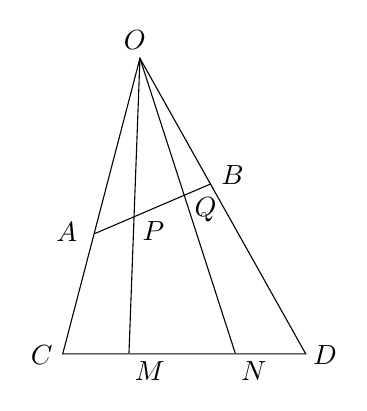
\begin{tikzpicture}[x=0.75pt,y=0.75pt,yscale=-1,xscale=1,scale=0.8]
			%uncomment if require: \path (0,300); %set diagram left start at 0, and has height of 300

			%Shape: Triangle [id:dp8404205470797059] 
			\draw   (322.17,54.17) -- (422,232.17) -- (275.67,232.17) -- cycle ;
			%Straight Lines [id:da9008684259134017] 
			\draw    (294.89,159.78) -- (364.89,129.78) ;
			%Straight Lines [id:da7092672100334034] 
			\draw    (322.17,54.17) -- (315.56,231.78) ;
			%Straight Lines [id:da3275050790851046] 
			\draw    (322.17,54.17) -- (379.56,231.78) ;

			% Text Node
			\draw (310.89,36.07) node [anchor=north west][inner sep=0.75pt]    {$O$};
			% Text Node
			\draw (270.22,151.73) node [anchor=north west][inner sep=0.75pt]    {$A$};
			% Text Node
			\draw (369.56,117.07) node [anchor=north west][inner sep=0.75pt]    {$B$};
			% Text Node
			\draw (254.89,225.73) node [anchor=north west][inner sep=0.75pt]    {$C$};
			% Text Node
			\draw (424.89,225.73) node [anchor=north west][inner sep=0.75pt]    {$D$};
			% Text Node
			\draw (317.56,235.18) node [anchor=north west][inner sep=0.75pt]    {$M$};
			% Text Node
			\draw (381.56,235.18) node [anchor=north west][inner sep=0.75pt]    {$N$};
			% Text Node
			\draw (322.22,151.07) node [anchor=north west][inner sep=0.75pt]    {$P$};
			% Text Node
			\draw (353.56,136.4) node [anchor=north west][inner sep=0.75pt]    {$Q$};


		\end{tikzpicture}
	\end{center}

	紧接着可问:

	(1)长度为1cm的线段上的点的个数与长度为100m的线段上的点的个数哪个多?

	(2)半径为1的圆周上点的个数与半径为2的圆周上点的个数哪个多?

	(3)正整数的个数与正偶数的个数一样多吗?

	(4)有理数与整数的个数一样多吗?

	(5)有理数与无理数的个数一样多吗?

	要告诉学生有理数与无理数是不一样多的,等到大学才能明白,这也是否定“无限多就是一样多的”的一个反例.
\end{example}
\begin{purpose}
	该例是高中第一章集合内容的拓展,通过该例让学生感悟到有限与无限之间有质的区别,在数学中部分可以等于整体,这在日常的生活中是不可思议的,因此本例是激发学生好奇心的很好素材.此外,希尔伯特旅馆的故事都可结合讲.
\end{purpose}
\begin{note}[希尔伯特旅馆\cite{XiErBoTeLuGuanBeiLun2023}]
	假设有一个拥有可数无限多个房间的旅馆,且所有的房间均已客满。或许有人会认为此时这一旅馆将无法再接纳新的客人(如同有限个房间的情况),但事实上并非如此。

	有限个新客人:设想此时有一个客人想要入住该旅馆。由于旅馆拥有无穷个房间,因而我们可以将原先在1号房间原有的客人安置到2号房间、2号房间原有的客人安置到3号房间,以此类推,这样就空出了1号房间留给新的客人。重复这一过程,我们就能够使任意有限个客人入住到旅馆内。

	无限个新客人:另外,我们还能使可数无限个新客人住到旅馆中:将1号房间原有的客人安置到2号房间、2号房间原有的客人安置到4号房间、n号房间原有的客人安置到2n号房间,这样所有的奇数房间就都能够空出来以容纳新的客人。
\end{note}

\begin{example}[杨辉三角]
	通过观察$(a+b),(a+b)^2,(a+b)^3,\ldots$ 展开式的各项系数,介绍杨辉三角.再尝试对 $(a+b)^5$ 的展开.
	\begin{equation*}
		\begin{array}{cccccccccc}
			  &   &   &   & 1      &   &   &   &   & \\
			  &   &   & 1 &        & 1 &   &   &   & \\
			  &   & 1 &   & 2      &   & 1 &   &   & \\
			  & 1 &   & 3 &        & 3 &   & 1 &   & \\
			1 &   & 4 &   & 6      &   & 4 &   & 1 & \\
			  &   &   &   & \cdots &   &   &   &   &
		\end{array}
	\end{equation*}
	本例是高中二项式定理中将介绍的杨辉三角(如图).杨辉三角又称贾宪三角形,帕斯卡三角形,是二项式系数在三角形中的一种几何排列.在欧洲,这个表叫做帕斯卡三角形.帕斯卡(1623—1662)是在1654年发现这一规律的,比杨辉要迟393年,比贾宪迟600年.
\end{example}
\begin{purpose}
	除展示数学结构美之外,渗透归纳思想,同时又渗透一下数学文化.
\end{purpose}

\begin{example}[极限雏形]
	当 $n \rightarrow \infty$ 时, $1+\frac{1}{2}+\frac{1}{3}+$ $\cdots+\frac{1}{n}$ 的值会不会超过 10?超过 100?超过 1 亿?

	有学生会认为超过 1 亿, 他相信积少成多的道理. 老师在肯定答案之时又马上给出变式: 当 $n \rightarrow \infty$时, $1+\frac{1}{2^2}+\frac{1}{3^2}+\cdots+\frac{1}{n^2}$ 的值会不会超过 10?超过 100? 超过 1 亿? 变化之后,连 2 都不会超过. 通过这种相似问题, 但结果又大相径庭, 从而引起学生的认知冲突, 从而激发学生对数学的探究欲望, 告诉学生,这些道理等以后学了极限就清楚了.
\end{example}
\begin{purpose}
	一让学生感受数列的收敛性和发散性, 二让学生再一次体会数学的奇异美.
\end{purpose}

\begin{example}[几何级数]
	电影《漂流瓶》中有一个故事,在船上有几位漂亮的女大学生,同时也有几位文化程度不高的男青年.在这些男青年中有一位绰号叫“三万”的,因为他有三兄弟,父母亲留给他们的财产共10万,平分后每人三万多点,故号称三万.其中一位女大学生想考考“三万”的才华,她说:“我跟你谈恋爱,有个条件:第1天给我1分钱,第2天给2分钱,第3天给4分钱,以后每天给的钱都是上一天的2倍.这样连续给一个月,如果给得起,我就同意.”而号称三万的青年认为这是毛毛雨,说可以,却不知道这是一个圈套.当用计算器按到第10天时,总共需要的钱只有10元2角4分,当按到第20天时,还行,1万多一点,而接下去就很快了,一个月下来给的钱总共大约需要2150多万.

	因为这个数列是成几何级数增长,增长速度之快是出乎人的常识之外.类似的还有折纸游戏,国王奖励国际象棋发明者的故事等等.
\end{example}
\begin{purpose}
	这个知识涉及到高中等比数列求和知识,另一点让学生明白知识的重要性.
\end{purpose}

\begin{example}[几何直觉]
	有两个三角形,其边长分别为17,25,26与17,25,28,求它们的内切圆半径谁大谁小.

	分析: 由 海 伦 公 式 $r=\sqrt{\frac{1}{p}(p-a)(p-b)(p-c)}, p=\frac{a+b+c}{2}$ 可算得: 以 $17,25,26$ 为边长的三角形的内切圆半径 $r_1=6$, 以 $17,25,28$ 为边长的三角形的内切圆半径 $r_2=6$.

	结果为 $r_1=r_2$, 完全出人意外! 估计百分之九十九的人会认为, 这两个三角形的内切圆半径虽然彼此相差不大, 但总应该有些微小差别, 绝对不会是相等的.
\end{example}
\begin{purpose}
	数学中直觉不一定可靠, 有时需要严密论证.
\end{purpose}

\begin{example}[数学悖论]
	一个理发师给自己立了这么一条店规:“只给那些不给自己刮脸的人刮脸.”那么,这位理发师的脸该不该由他自己刮?

	如果理发师的脸由他自己刮,则他属于“自己给自己刮脸的人.”因此,理发师不应该给自己刮脸;如果理发师的脸不由他自己刮,则他又属于“自己不给自己刮脸的人.”因此,他的脸可由自己刮,这显然又与上述“自己不给自己刮脸的人”相矛盾.从以上分析,这样不对,那样也不对,就是数学中的悖论.
\end{example}
\begin{purpose}
	激发学生对数学逻辑的兴趣,同时也可介绍数学发展的几次危机.
\end{purpose}
\begin{note}[数学危机\cite{ShuXueWeiJi2023}]
	数学危机在历史上发生过三次,每一次均对数学的发展有重大影响。在第一次数学危机中,因为发现腰长为1的等腰直角三角形的斜边长度无法写成有理数,从而引申出日后的无理数概念。第二次数学危机得以解决微积分引入无穷小量而产生的问题。第三次数学危机则是因罗素悖论而起,它点出朴素集合论中的缺失。
\end{note}
\subsection{例说高中数学之重要}
做一件事光有兴趣是远远不够的,只有认识到做这件事的意义和重要性,才能有做好这件事不竭的动力,学习数学也是一样.数学学科是一门基础学科,它的重要性是多方面、多角度、多层次的.

1. 数学是一种描述自然的语言.

数学语言刻画事物的数量关系、形式与形状,反映事物的本质属性.当人们需要把客观事物的认识精确化的时候,必须使用数学语言. 诺贝尔物理学奖获得者菲曼曾说:“要是没有数学语言,宇宙几乎是不可描述的!”例如,牛顿用数学公式展示了物质运动的三大定律,爱因斯坦用黎曼有关弯曲空间曲率理论阐述广义相对论;化学家、生物学家、经济学家等都必须用数学语言使自己的学科精密化.

2.数学是培养思维能力的重要载体.

法国数学家格瑞斯曼说过这样的话:“数学除了锻炼敏锐的理解力,发现真理外,它还有另一个训练全面考虑和科学系统的头脑的开发功能.”

通过数学学习,形成一种数学思想和能力,明确数量观念,注意事物的数量关系与变化规律;通过数学学习,了解数学的概念、方法、理论等的产生和发展的渊源及过程,了解和领会从实际出发建立数学模型,再到解决问题的全过程;通过数学学习,提高人的逻辑思维能力,能在纷繁复杂的各项工作面前有条不紊地处理等.

\begin{example}
	甲、乙二人在一圆形桌面上轮流放面值一样的硬币,不可重叠,当谁放不下了,谁就输.如果甲先放,问有无必胜的策略?
\end{example}

\begin{analysis}
	如果甲、乙二人随意去放,显然甲不一定能赢.但如果能从数学对称原理去想,先放者就有必胜的策略.只要甲第一次先放在桌子的中心,接下来乙放,然后甲放在乙刚放的关于圆心的对称点上,依次下去,由对称原理,只要乙能放,甲肯定能放,故甲胜.

	本题将随意放硬币的游戏进行有序化,先夺取“战略高地”,这就是数学的思维.
\end{analysis}

\begin{example}
	证明: 任意6人中,至少有3人两两相互认识或两两互不认识.
\end{example}

\begin{analysis}
	这一问题如果将各种情况都加以考虑,也是一种思路,穷举法,但情况比较多,显得繁杂.现在将问题进行数学化,就不难了.将6人视为平面上6个点,相互认识的用实线相连,相互不认识的用虚线相连.

	先考虑从A点出发与其它五个点连线情况,共有5条线,由于只有实线与虚线二种情形,因此由抽屉原理可以断定这5条线中至少有3条是同一类型的,譬如,有3条实线AB,AC,AE,现在分析B,C,E三点之间的连线,若B,C,E三点之间的连线有一条是实线,譬如BE,那么A,B,E三者的连线都是实线,问题解决,反之,若B,C,E三点之间的连线都是虚线,问题也得证.
\end{analysis}

3.数学是科学技术进步的直接推手

我国著名数学家华罗庚先生曾说:“宇宙之大,粒子之微,火箭之速,化工之巧,地球之变,生物之谜,日用之繁等各个方面,无处不有数学.”由此可见数学应用是非常广泛的.

二十世纪科学技术进步给人类生产和生活带来的巨大变化确实令人赞叹不已.从远古时代起一直是人们幻想的“顺风耳”、“千里眼”、“空中飞行”和“飞向太空”都在这一世纪成为现实.回顾二十世纪的重大科学技术进步,以下几个项目无疑是影响最大的,而数学的预见和推动作用是非常关键.

(1)先有了麦克斯韦方程,人们从数学上论证了电磁波,其后赫兹才有可能做发射电磁波的实验,接着才会有电磁波声光信息传递技术的发展.

(2)爱因斯坦相对论的质能公式首先从数学上论证了原子反应将释放出的巨大能量,预示了原子能时代的来临.随后人们才在技术上实现了这一预见,到了今天,原子能已成为发达国家电力能源的主要组成部分.

(3)牛顿当年已经通过数学计算预见了发射人造天体的可能性,差不多过了将近三个世纪,人们才实现了这一预见.

(4)电子数字计算机的诞生和发展完全是在数学理论的指导下进行的.数学家图灵和冯诺依曼的研究对这一重大科学技术进步起了关键性的推动作用.

(5)遗传与变异现象虽然早就为人们所注意.生产和生活中也曾培养过动植物新品种.遗传的机制却很长时间得不到合理解释,十九世纪60年代,孟德尔以组合数学模型来解释他通过长达8年的实验观察得到的遗传统计资料,从而预见了遗传基因的存在性.多年以后,人们才发现了遗传基因的实际承载体,到了本世纪50年代沃森和克里发现了DNA分子的双螺旋结构.这以后,数学更深刻地进入遗传密码的破译研究.

数学是人类理性思维的重要方式,数学模型,数学研究和数学推断往往能作出先于具体经验的预见.这种预见并非出于幻想而是出于对以数学方式表现出来的自然规律和必然性的认识,随着科学技术的发展,数学、预见的精确性和可检验性日益显示其重意义.

\subsection{高中数学与初中数学的差异}
1. 知识差异

初中: 内容少、浅、面窄,常量为主, 题型少、简单,可反复磨炼,甚至死记硬背就可以考出高分.

高中:知识多、深、面宽;变量为主, 题型多, 没有时间反复.

2. 教法差异

初中: 课堂容量小,讲速慢,题型少,反复,模仿.

高中: 课堂容量大,知识复杂,速度快,题型多,很少反复.

3. 学法差异

初中: 自学能力差, 讲授, 被动学, 反复练.

高中:自主探索, 主动学习, 获得知识的渠道宽.

4.语言差异

初中:初中的数学主要是以形象、通俗的语言方式进行表达.

高中: 高一进来就触及抽象的集合符号语言、逻辑运算语言、函数语言、图形语言等, 也就是说抽象化程度大大提升,抽象是感觉难的主要原因.

5.思维差异

初中:很多老师为学生将各种题型建立了统一的思维模式(如:解分式方程分几步;因式分解先看什么、再看什么,等等),确定了常见的思维套路,因此,形成初中阶段在数学学习中习惯于这种机械的、便于操作的定式.

高中:在解题方法步骤上灵活多变,往往能一题多解,用代数法能解出,用几何法也能解出,但每种解题方法所用时间和出错的机会不一样,这就要求对各种思想方法如数形结合、分类讨论、整体换元、消元等思想方法融会贯通,思想方法的学习就像外语的语法一样,在高中数学的学习中占很大比例.

\subsection{高中数学学习方法}
(一)高中数学的学习方法六字方针:思考,运算,积累.

1.思考是核心.

学数学有时课堂上都能听懂,老师讲的题目觉得自己都会,可是课下自己一做就错,有的问题甚至没有思路.学数学最忌讳的是老师讲同学听,听完之后做笔记,从头听到尾,从头记到尾,听的特明白,笔记记得特清楚,轮到自己一做题还是不会做,还是无处下手,这就好比同学们站在岸上学游泳,没有经过那个被水淹、在水里扑腾的过程,老师示范的再清楚你还是白搭.要将思考贯穿于数学学习的整个过程,无论课上老师的提问,还是课下自己做题,我们始终要做的就是思考:为什么这样做,为什么要这样变形,这道题还能怎么做,这类题目解决的共同方法是什么,所蕴含的思想方法是什么,等等.数学学习的主阵地是课堂,老师提出问题后同学们的大脑就要飞速地旋转,哪怕有一点点思路也要积极回答,这样积极参与的过程学习效率很高.

2.运算是基础.

数学离不开算.在小学阶段被称为算术,初中阶段被称为代数,用字母代替数字进行运算,在高中更是通过指数、对数、三角函数、向量、排列组合、算法等载体发展人的计算能力.较复杂的解析几何题目运算过程可达几十步,只要错了一个正负号或算错一个小数就会满盘皆输,整个大题报废,离开了一个强大的计算能力就谈不上学好数学.所以说,一道题从有了思路到完整解答还差多少里?十万八千里!为了提高计算能力,在笔算的基础上更要心算.学数学要将算放在首位,这也是对数学的第一个也是最重要的一项要求.运算是能力,能力的提升没有什么巧妙的方法,就是要拿出你的耐心和细心大量地练,亲自动手将每一个得数算出来,当然还要掌握好算理.

3.积累是保障.

数学课如果有几节课没听,有几节练习没跟着做,再接着听便不好听懂,甚至一点都不会.由此可见数学的一个重要特点就是必须将先学的知识彻底掌握才能进行后续的学习.前边提到数学的一个重要特点就是抽象,内容都是用字母和符号表达的,这就要求同学们必须对学过的东西进行持之以恒的反复记忆和运算,通过这种方式将抽象的东西内化,最后形成直觉.但数学题太多了,人们都把它比喻成题海,都记不把人累死吗?这就涉及到积累什么东西的问题.牵牛要牵鼻子,想问题办事情要抓关键,抓主要矛盾.高中数学的这个关键就是指好题:有代表性的,通过这道题能掌握好几个重要知识点,能掌握解一类问题的通法,能以一顶十的题目.要是让你单纯背诵你总觉得这事有点荒唐,不像文科的东西那样好背,或者说根本就不适合背诵,怎么办?多做,好题做六遍,做的遍数多自然就掌握了.所以我们要积累的东西是上课老师所讲授的典型例题,解决典型例题的思想方法.课上要逐渐学会迅速记录简明的课堂笔记,课下详细整理,补充详实.除此之外还有学着整理做过的试卷,这些试卷上往往有很多精彩的题目,都往笔记本上誊写没那时间,索性直接将笔记做在卷子上,每隔一段时间进行阅读,尤其是考前这么做效果最好.

(二)五点建议

1.认真听好每一节课

有的同学上课不听,下课不看,资料不做,考试前拿着课本在那记公式,总结知识点,考试成绩是一塌糊涂.原因是什么?为什么初中可以考前突击,现在却不行了?初中知识简单,结构单一,高中数学灵活多变,不是靠死记硬背,更多的是课堂上讲解的解题的思想方法.

2.做好数学笔记

特别是对概念不同侧面的理解,以及典型例题.

3. 建立数学错题本

把平时容易出现错误的知识或推理记载下来,以防再犯.争取做到:找错、析错、改错、防错.达到:能从反面入手深入理解;能由果溯因把错误原因弄个水落石出、以便对症下药;解答问题完整、推理严密.

4. 记忆数学规律和数学小结论

高中数学不是靠死记硬背,但是不代表不背,基本的规律和结论还是必须记的,记的熟练了,自然也就能灵活运用了.

5. 学会总结归类

(1)从数学思想分类;(2)从解题方法归类;(3)从知识应用上分类.

\begin{note}
	个人按照时间顺序的三点建议:
	\begin{enumerate}
		\item     课前——做好预习,提前阅读教材并完成全品“课前预习”部分,了解将要学习的内容,不懂的地方做好标记,带着问题上课;
		\item 课堂——集中精力听讲,积极参与课堂讨论,及时记笔记。对于不理解的部分,课后及时解决;
		\item 课后——及时复习当天内容,先自己复习梳理一遍当天所学知识再写作业,按时提交作业,建立数学错题本,学会总结归纳.
	\end{enumerate}
\end{note}

本文从四个方面设计高中数学起始课,由于内容多,建议用两种方式灵活处理,一是上两节课;二是精简内容,并结合教师自己的特长与兴趣进行设计.

\section{乘法公式与因式分解}
\marginnote{2024-7-23}
\subsection{归纳初中知识}
在初中, 我们学习了多项式的乘法运算, 知道乘法公式可以使多项式的运算变得更为简便. 初中主要学习了两个基本的乘法公式一平方差公式和完全平方公式.
\begin{formula}[平方差公式]
	$(a+b)(a-b) = a^2-b^2$.
\end{formula}

\begin{formula}[完全平方公式]
	$(a\pm b)^2 = a^2  \pm 2ab + b^2$.
\end{formula}

\subsection{衔接高中知识}
高中代数部分是以函数为主线展开学习的,为研究函数的性质, 需要同学们具有较强的代数恒等变形能力, 也就是说,在高中学习中还会遇到更为复杂的多项式的乘法运算. 因此, 在本节中,我们将拓展乘法公式的内容,补充一些高中常用的乘法公式.

由于
\begin{align}
	(a+b)^3 & =(a+b)^2(a+b)=\left(a^2+2 a b+b^2\right)(a+b) \\
	        & =a^3+a^2 b+2 a^2 b+2 a b^2+a b^2+b^3          \\
	        & =a^3+3 a^2 b+3 a b^2+b^3 .
\end{align}

于是有
\begin{formula}[完全立方和公式]
	$(a+b)^3=a^3+3 a^2 b+3 a b^2+b^3$.
	\label{完全立方和公式}
\end{formula}

将\autoref{完全立方和公式}中的 $b$ 全部换成 $-b$, 得到完全立方差公式:
\begin{formula}[完全立方差公式]
	$(a-b)^3=a^3-3 a^2 b+3 a b^2-b^3$.
\end{formula}

由完全立方和公式可得 $(a+b)^3-3 a^2 b-3 a b^2=a^3+b^3$, 即 $(a+b)\left[(a+b)^2-3 a b\right]=a^3+b^3$.
于是有
\begin{formula}[立方和公式]
	$a^3+b^3=(a+b)\left(a^2-a b+b^2\right)$.
\end{formula}

同理,由完全立方差公式可得 $(a-b)\left[(a-b)^2+3 a b\right]=a^3-b^3$, 即
\begin{formula}[立方差公式]
	$a^3-b^3=(a-b)\left(a^2+a b+b^2\right)$.
\end{formula}
由于
\begin{align}
	(a+b+c)^2 & =[(a+b)+c]^2=(a+b)^2+2(a+b) c+c^2 \\
	          & =a^2+2 a b+b^2+2 a c+2 b c+c^2    \\
	          & =a^2+b^2+c^2+2 a b+2 a c+2 b c .
\end{align}

于是有
\begin{formula}
	$(a+b+c)^2=a^2+b^2+c^2+2 a b+2 a c+2 b c$.
\end{formula}

同时,我们还应注意乘法公式的一些常见变形:
\begin{enumerate}
	\item $a^2+b^2=(a+b)^2-2 a b$;
	\item $a^2+b^2=(a-b)^2+2 a b$;
	\item $(a+b)^3=a^3+b^3+3 a b(a+b)$;
	\item $a^3+b^3=(a+b)^3-3 a b(a+b)$.
\end{enumerate}

\subsection{精讲典型例题}
\begin{example}
	已知 $x+y=-5, xy=6$, 求 $x^2+y^2$ 的值.
\end{example}
\begin{analysis}
	利用完全平方公式的变形 $a^2+b^2=(a+b)^2-2 a b$ 进行求解.
\end{analysis}
\begin{solution}
	\begin{align*}
		\because x+y=-5,   & x y=6.             \\
		\therefore x^2+y^2 & =(x+y)^2-2 x y     \\
		                   & =(-5)^2-2 \times 6 \\
		                   & =13 .
	\end{align*}
\end{solution}

\begin{example}
	分解因式: $8 x^3+27 y^3+36 x^2 y+54 x y^2$.
\end{example}
\begin{solution}
	\begin{align}
		  & 8 x^3+27 y^3+36 x^2 y+54 x y^2                                   \\
		= & 8 x^3+36 x^2 y+54 x y^2+27 y^3 \quad (\text{按}x\text{降幂排列}) \\
		= & (2 x)^3+3(2 x)^2(3 y)+3(2 x)(3 y)^2+(3 y)^3                      \\
		= & (2 x+3 y)^3 .
	\end{align}
\end{solution}

\begin{example}
	分解因式: $a^6+b^6$.
\end{example}
\begin{solution}
	\begin{align}
		  & a^6+b^6                                                                        \\
		= & \left(a^2\right)^3+\left(b^2\right)^3                                          \\
		= & \left(a^2+b^2\right)\left[\left(a^2\right)^2-a^2 b^2+\left(b^2\right)^2\right] \\
		= & \left(a^2+b^2\right)\left(a^4-a^2 b^2+b^4\right) .
	\end{align}
\end{solution}

\begin{example}
	分解因式: $a^6-b^6$.
\end{example}
\begin{solution}
	$a^6$ 可以看成平方:
	\begin{align*}
		a^6=\left(a^3\right)^2,
	\end{align*}
	也可以看成立方:
	\begin{align*}
		a^6=\left(a^2\right)^3,
	\end{align*}
	于是 $a^6-b^6$ 的分解就有两条路可走.
	第一条路是先应用平方差公式:
	\begin{align*}
		  & a^6-b^6                                                      \\
		= & \left(a^3\right)^2-\left(b^3\right)^2                        \\
		= & \left(a^3+b^3\right)\left(a^3-b^3\right)                     \\
		= & (a+b)\left(a^2-a b+b^2\right)(a-b)\left(a^2+a b+b^2\right) .
	\end{align*}
	第二条路是从立方差公式入手:
	\begin{align*}
		  & a^6-b^6                                          \\
		= & \left(a^2\right)^3-\left(b^2\right)^3            \\
		= & \left(a^2-b^2\right)\left(a^4+a^2 b^2+b^4\right) \\
		= & (a+b)(a-b)\left(a^4+a^2 b^2+b^4\right) .
	\end{align*}
	采用两种方法分解, 获得的结果应当相同. 因此比较
	\begin{align*}
		(a+b)\left(a^2-a b+b^2\right)(a-b)\left(a^2+a b+b^2\right)
	\end{align*}
	与
	\begin{align*}
		(a+b)(a-b)\left(a^4+a^2 b^2+b^4\right),
	\end{align*}

	我们知道 $a^4+a^2 b^2+b^4$ 不是既约多项式, 并且有
	\begin{align*}
		a^4+a^2 b^2+b^4=\left(a^2+a b+b^2\right)\left(a^2-a b+b^2\right)
	\end{align*}
	及
	\begin{align*}
		a^6-b^6=(a+b)(a-b)\left(a^2+a b+b^2\right)\left(a^2-a b+b^2\right) .
	\end{align*}
\end{solution}

\begin{example}
	当 $a+b+c=0, a^2+b^2+c^2=1$ 时, 求下列各式的值.

	(1) $b c+c a+a b$;

	(2) $a^4+b^4+c^4$.
\end{example}
\begin{analysis}
	将 (1) 与已知联系, 联想已知中的等式, 发现可将 $b c+$ $c a+a b$ 用 $a+b+c$ 和 $a^2+b^2+c^2$ 表示. 由于 $a^4+b^4+c^4=\left(a^2\right)^2+$ $\left(b^2\right)^2+\left(c^2\right)^2$. 由 (1)得到启示, 如果知道 $a^2 b^2+b^2 c^2+c^2 a^2$ 的值, 就能得解.
\end{analysis}
\begin{solution}
	(1) $\because(a+b+c)^2=a^2+b^2+c^2+2(a b+b c+c a)$
	且 $a+b+c=0, a^2+b^2+c^2=1$,

	$\therefore 0^2=1+2(a b+b c+c a),$

	即 $b c+c a+a b=-\frac{1}{2}$.

	(2)	\begin{align}
		 & \because(b c+c a+a b)^2                                        \\
		 & =b^2 c^2+c^2 a^2+a^2 b^2+2\left(a^2 b c+a b^2 c+a b c^2\right) \\
		 & =b^2 c^2+c^2 a^2+a^2 b^2+2 a b c(a+b+c),                       \\
		 & \therefore b^2 c^2+c^2 a^2+a^2 b^2=\frac{1}{4} .
	\end{align}
	$ \therefore a^4+b^4+c^4=\left(a^2\right)^2+\left(b^2\right)^2+\left(c^2\right)^2+2 a^2 b^2+2 b^2 c^2+2 c^2 a^2 \\
		=1+2 \times \frac{1}{4}=\frac{3}{2} .$
\end{solution}

\begin{example}
	求证 $2^{1984}+1$ 不是质数\cite{DanDunShuXueAoLinPiKeXiaoCongShuChuZhongJuanYinShiFenJieJiQiao2005}.
\end{example}
为了将 $2^{1984}+1$ 分解因数, 我们需要知道一个新的公式, 即在 $n$ 为\textbf{正奇数}时, 有
\begin{formula}
	\begin{align}
		a^n+b^n=(a+b)\left(a^{n-1}-a^{n-2} b+a^{n-3} b^2-\cdots-a b^{n-2}+b^{n-1}\right) .
	\end{align}
\end{formula}
\begin{proof}
	上式不难用乘法验证, 将右边的两个因式相乘便得到 $a^n+b^n$.现在我们有
	\begin{align}
		  & 2^{1984}+1                                                                            \\
		= & \left(2^{64}\right)^{31}+1^{31}                                                       \\
		= & \left(2^{64}+1\right)\left(2^{64 \times 30}-2^{64 \times 29}+\cdots-2^{64}+1\right) .
	\end{align}
	$2^{64}+1$ 是 $2^{1984}+1$ 的真因数, 它大于 1 , 小于 $2^{1984}+1$, 所以 $2^{1984}+1$ 不是质数.
\end{proof}
用上述方法可以证明: 当 $n$ 有大于 1 的奇数因数时, $2^n+1$ 不是质数. 类似地, 由乘法可以得到在 $n$ 为\textbf{正整数}时有
\begin{formula}
	\begin{equation}
		a^n-b^n=(a-b)\left(a^{n-1}+a^{n-2} b+a^{n-3} b^2+\cdots+a b^{n-2}+b^{n-1}\right) .
	\end{equation}
\end{formula}
这也是一个有用的公式.

\begin{example}
	分解因式: $x^5-1$.
\end{example}
\begin{solution}
	$x^5-1=(x-1)\left(x^4+x^3+x^2+x+1\right)$.
\end{solution}
\begin{note}
	上面两道例题蕴含了特殊到一般的数学思想方法.
\end{note}

\section{根式及其运算}
\marginnote{2024-7-24}
\subsection{归纳初中知识}
在初中, 我们主要学习了二次根式的概念及其运算.
\begin{enumerate}
	\item 二次根式定义中 $\sqrt{a}(a \geqslant 0)$ 是一个整体, 表示非负数 $a$ 的算术平方根. 在实数范围内对负数不能施行开平方运算, 故 $a \geqslant 0$ 这个条件必不可少.
	\item $(\sqrt{a})^2=a(a \geqslant 0), \sqrt{a^2}=|a|=\left\{\begin{array}{l}a(a>0), \\ 0(a=0), \\ -a(a<0) .\end{array}\right.$
	      \begin{enumerate}
		      \item $(\sqrt{a})^2(a \geqslant 0)$ 的运算顺序是先求一个非负数的算术平方根, 然后再平方. 注意必须满足 $a \geqslant 0$ 的条件.
		      \item $\sqrt{a^2}$ 的运算顺序是先平方再开方, 取算术平方根. 故此式对任何实数都有意义. 使用公式时注意 $\sqrt{a^2}=|a|$ 的应用.
		      \item 化简过程中一定要注意符号问题. 当性质 $\sqrt{a^2}=-a(a<0)$ 逆运用时应是 $a=-\sqrt{a^2}$ $(a<0)$, 即把负数 $a$ 移到根号里面时, 应把“一”号留在根号外面.
	      \end{enumerate}
	\item 二次根式具有非负性, 即 $\sqrt{a} \geqslant 0(a \geqslant 0)$.
\end{enumerate}

\subsection{衔接高中知识}
高中在二次根式的基础上研究 $n$ 次根式, 学习 $n$ 次根式和分数指数幂的互化以及根式的运算, 另外高中解无理方程、解无理不等式、建立圆雉曲线的方程等, 都需要对二次根式的运算非常焦练、灵活.
\subsubsection{$n$ 次根式}
实际上, 数的平方根的概念可以推广. 一般地, 如果 $x^{n}=a$, 那么$x$叫做 $a$ 的 $n$ 次方根. 例如, 由于 $2^4=16$ 和 $(-2)^4=16$, 我们把 $2$ 或 $-2$ 叫做 $16$ 的 $4$ 次方根. 当 $n$ 是偶数时, 正数 $a$ 的正的 $n$ 次方根用符号 $\sqrt[n]{a}$ 表示, 负的 $n$ 次方根用符号 $-\sqrt[n]{a}$ 表示, 也可以把两个方根合起来写作 $\pm \sqrt[n]{a}$. 例如, $\sqrt[4]{16}=2,-\sqrt[4]{16}=-2$, 合起来写作 $\pm \sqrt[4]{16}= \pm 2$.
类比二次根式的性质, 我们得到$n$次根式的性质:
\begin{enumerate}
	\item $(\sqrt[n]{a})^{n}=a\left(n \in \mathbb{N}^*\right)$. 特别地, $(\sqrt{a})^2=a(a \geqslant 0),(\sqrt[3]{a})^3=a(a \in \mathbb{R})$.
	\item 当 $n$ 是正奇数时, $\sqrt[n]{a^n}=a$; 当 $n$ 是正偶数时, $\sqrt[n]{a^n}=|a|$. 特别地, $\sqrt{a^2}=|a|=$ $\left\{\begin{array}{l}a, a \geqslant 0, \\ -a, a<0, \\ \sqrt[3]{a^3}=a(a \in \mathbb{R}) .\end{array}\right.$
	\item $\sqrt[n]{a}=a^{\frac{1}{n}}\left(a>0, n>1, n \in \mathbb{N}^*\right) ; \frac{1}{a^n}=a^{-n}\left(a \neq 0, n \in \mathbb{N}^*\right)$.
\end{enumerate}
\subsubsection{分母(分子)有理化}
分母有理化的方法是分母和分子都乘以分母的有理化因式, 化去分母中的根号的过程. 在高中数学中, 有时需要把分式的分子进行有理化, 即分式的分子和分母都乘以分子的有理化因式, 化去分子中的根号.

\subsection{精讲典型例题}
\begin{example}
	有理化下列各式的分子:

	(1) $\frac{\sqrt{x+1}+\sqrt{x}}{\sqrt{x+1}-\sqrt{x}}$;

	(2) $\frac{a-1+\sqrt{a^2-1}}{a+1+\sqrt{a^2-1}}(a>1)$.
\end{example}
\begin{analysis}
	$\sqrt{x+1}+\sqrt{x}$ 有理化因式为 $\sqrt{x+1}-\sqrt{x}$, (2) 可先化简约分.
\end{analysis}
\begin{solution}
	(1)
	\begin{align}
		\text{原式} & =\frac{(\sqrt{x+1}+\sqrt{x})(\sqrt{x+1}-\sqrt{x})}{(\sqrt{x+1}-\sqrt{x})^2} \\
		            & =\frac{x+1-x}{(\sqrt{x+1}-\sqrt{x})^2}=\frac{1}{(\sqrt{x+1}-\sqrt{x})^2} .
	\end{align}
	(2)
	\begin{align}
		  & \frac{a-1+\sqrt{a^2-1}}{a+1+\sqrt{a^2-1}}                                   \\
		= & \frac{\sqrt{(a-1)^2}+\sqrt{(a+1)(a-1)}}{\sqrt{(a+1)^2}+\sqrt{(a+1)(a-1)}}   \\
		= & \frac{\sqrt{a-1}(\sqrt{a-1}+\sqrt{a+1})}{\sqrt{a+1}(\sqrt{a+1}+\sqrt{a-1})} \\
		= & \frac{\sqrt{a-1}}{\sqrt{a+1}}=\frac{a-1}{\sqrt{a^2-1}} .
	\end{align}
\end{solution}

\section{无理方程}
\marginnote{2024-7-24}
\subsection{归纳初中知识}
初中我们已经学习了整式、分式、根式的概念, 学习了一元一 (二)次方程、简单二元一次方程组和可化为一元一 (二) 次方程的分式方程 (方程中的分式不超过两个)的解法, 但没有涉及无理方程的解法, 在高中新课程的函数、三角和不等式的学习以及立体几何初步和平面解析几何初步学习中又要经常用到这部分的知识, 为了高中学习顺利, 本专题重点介绍无理方程 (含二次根式)的解法, 希望大家能够掌握.

\subsection{衔接高中知识}
根号下含有未知数的方程, 叫做无理方程.
解无理方程的基本思想: 去 “根号”, 化无理方程为有理方程再求解.

解无理方程的基本方法: 平方法, 即方程两边平方化无理方程为有理方程求解, 遇到平方后次数比二次大的较复杂的无理方程可尝试用换元法求解.
特别注意: 解无理方程最后要验根.

\subsection{精讲典型例题}
\begin{example}
	解方程 $\sqrt{3 x-5}-\sqrt{x+2}=1$.
\end{example}
\begin{analysis}
	方程左边有两个二次根式, 如果直接平方, 结果较繁, 一般把其中一个根式移到方程的右边, 使方程左右两边各含有一个根式。
\end{analysis}
\begin{solution}
	移项, 得 $\sqrt{3 x-5}=\sqrt{x+2}+1$,

	两边平方, 得 $3 x-5=1+2 \sqrt{x+2}+x+2$,

	化简, 得 $x-4=\sqrt{x+2}$,

	两边再平方并整理, 得 $x^2-9 x+14=0$,

	解得 $x_1=2, x_2=7$.

	经检验, $x=2$ 是增根, $x=7$ 是原方程的根.
\end{solution}

\begin{example}
	设实数 $x>0$, 求使等式
	\begin{align*}
		\sqrt{x^2-1}+\sqrt{x^2+4 x+3}=\sqrt{3 x^2+4 x+1}
	\end{align*}
	成立的所有 $x$ 的值\cite{葛军2012数学奥林匹克小丛书}.
\end{example}
\begin{analysis}
	观察等式即知方程的各项中都有式子 $\sqrt{x+1}$ (因为 $x>0$, 得 $x+1>0$ ), 从而转化原方程为 $\sqrt{x+1}=0$ 和 $\sqrt{x-1}+\sqrt{x+3}=\sqrt{3 x+1}$. 然后, 逐步去根号转化为易求解的方程.
\end{analysis}
\begin{solution}
	$\sqrt{(x+1)(x-1)}+\sqrt{(x+1)(x+3)}=\sqrt{(3 x+1)(x+1)}$.
	
	因为 $x>0$, 所以 $x+1>0$, 从而知 $x-1 \geqslant 0, x+3>0,3 x+1>0$,于是有 $\sqrt{x+1}=0$ 或 $\sqrt{x-1}+\sqrt{x+3}=\sqrt{3 x+1}$.
	
	由 $\sqrt{x+1}=0$ 得 $x_1=-1$.
	
	由 $\sqrt{x-1}+\sqrt{x+3}=\sqrt{3 x+1}$, 两边平方整理得
	\begin{align*}
		2 \sqrt{(x-1)(x+3)}=x-1 .
	\end{align*}

	从而有 $\sqrt{x-1}=0$ 或 $2 \sqrt{x+3}=\sqrt{x-1}$, 于是 $\sqrt{x-1}=0$ 得 $x_2=1$,由 $2 \sqrt{x+3}=\sqrt{x-1}$ 得 $x_3=-\frac{13}{3}$.
	经检验, $x=1$ 为符合题中要求的 $x$.
\end{solution}
\begin{note}
	还可以直接通过平方逐次去根号转化为多项式方程求解. 若用此方法, 则题中条件 $x>0$ 可去掉.
\end{note}

\begin{example}
	解方程 $2 x^2+3 x+3=5 \sqrt{2 x^2+3 x+9}$.
\end{example}
\begin{analysis}
	$\sqrt{2 x^2+3 x+9}$ 是 $2 x^2+3 x+9$ 的算术平方根, 如果直接平方, 结果很繁, 若设 $\sqrt{2 x^2+3 x+9}=y$, 则原方程可转化为 $y$ 的一元二次方程.
\end{analysis}
\begin{solution}
设 $\sqrt{2 x^3+3 x+9}=y$, 则平方后得 $2 x^2+3 x=y^2-9$,原方程可化为 $y^2-9+3=5 y$, 即 $y^2-5 y-6=0$.
解这方程得 $y=6$ 或 $y=-1$.

当 $y=-1$ 时, $\sqrt{2 x^2+3 x+9}=-1$ 没有意义,无解, 舍去.

当 $y=6$ 时, $\sqrt{2 x^2+3 x+9}=6$,

解方程得 $x=3$ 或 $x=-\frac{9}{2}$.

检验: 把 $x=-\frac{9}{2}$ 代入原方程, 左边 $\neq$ 右边, 所以 $x=-\frac{9}{2}$ 为原方程的增根.

把 $x=3$ 代入原方程, 左边 $=30=$ 右边, 所以 $x=3$ 是原方程的解.

$\therefore$ 原方程的解为 $x=3$.
\end{solution}

\chapter{集合与常用逻辑用语}
\section{集合的概念}
\marginnote{2024-7-31}
\subsection{教材分析与教学重难点}
重点: 元素与集合的"属于"关系, 用符号语言刻画集合.

难点: 用描述法表示集合.
\subsection{教学目标}
\begin{enumerate}
	\item 通过示例,了解集合的含义,理解元素与集合的属于关系.
	\item 对于具体问题,能在自然语言和图形语言的基础上,用符号语言表示集合.
	\item 在具体情境中,了解全集与空集的含义.
\end{enumerate}
\subsection{学情分析}

\subsection{教学方法}

\subsection{板书设计}
\begin{boardenv}[集合的概念]
	\begin{enumerate}
		\item 集合的概念\\
		      一般地,我们把研究对象看作是\textbf{元素},把一些元素组成的整体看作是一个\textbf{集合}.
		\item 性质\\
			  确定性、互异性
		\item 属于关系\\
		      $a$属于集合$A$: $a\in A$\\
		      $a$不属于集合$A$: $a\notin A$.
		\item 集合的表示方法\\
		      描述法\\
		      列举法
	\end{enumerate}
\end{boardenv}



\subsection{教学过程}
\begin{intro}[教学片段\cite{HouCongShuXueHaoWanDaoWanHaoShuXueGaoZhongShuXueDiYiKeBuFangCongWan2020}]
	面对新的教师,新的同学,学生往往比较拘谨,不敢表达,这无疑会影响教师教育教学的质量.故而,教师在课程导入时,不妨以集合的“确定性”为背景和学生开一个小玩笑.班长:起立!学生:老师好!教师笑语:同学们好!请所有长头发的同学站一下,其余同学请坐下.(停顿几秒给学生思考)教师继续:(目测包含所有站着的学生)请站着的同学中身高低于2米的坐下.
\end{intro}
\begin{purpose}
	意在建立学生对集合概念的感性认识.“长头发”的不确定性引发学生思考:多长的头发算长头发?部分头发较长的女生不知所措,有的男生也在纠结自己的坐与站的问题.教师快速追加坐下的条件“身高低于2米”,则所有站立的学生坐下,化解了这一部分学生的尴尬.课堂上,师生谈笑间拉近了心理的距离.
\end{purpose}

\begin{intro}
	教师开始本节课的导入语:首先祝贺大家升入高中的学习,老师刚刚以高中数学中“集合”的概念为背景和大家开了一个小玩笑.什么是集合?我们全班的全体同学可以是一个集合,全体的男同学或全体的女同学也都是一个集合,但所有长头发的同学不能构成一个集合,因为集合要满足其内在的个体(元素)是确定的.这也是引发部分同学不确定自己是坐还是站的原因,而站着的同学中“身高低于2米的同学”显然是能够确定的,它是一个集合.集合是现代数学的一个基本概念,也是我们高中数学学习的第一个概念.同学们在后续的学习中要注意数学概念的学习,概念的理解程度决定了我们数学学习的深度,也直接决定了数学解题水平的高低.
\end{intro}
\begin{purpose}
	通过学生不难理解的集合概念,让学生体会数学概念在数学学习中的重要性.教学中,教师不必对集合的概念加以定义,以学生的感性认识理解即可,意在提升学生的学习兴趣和数学认知,也可留下悬念为后续正式学习集合相关知识铺垫情感因素.
\end{purpose}

\subsection{归纳总结与作业布置}
\section{集合的表示方法}
\subsection{教材分析与教学重难点}

\subsection{教学目标}

\subsection{学情分析}

\subsection{板书设计}

\subsection{教学过程}

\subsection{归纳总结与作业布置}

\section{集合的基本运算}
\subsection{教材分析与教学重难点}

\subsection{教学目标}

\subsection{学情分析}

\subsection{板书设计}

\subsection{教学过程}

\subsection{归纳总结与作业布置}

\section{}
%\chapter{一元二次函数、方程和不等式}

%\chapter{函数的概念与性质}

%\chapter{指数函数与对数函数}
\section{指数函数的图象与性质}\marginnote{2024-7-8}
\subsection{教材分析}
《指数函数的图象与性质》选自人教A版必修一函数部分第四章第二节,在此之前,学生已经学过了幂函数的图象与性质,而接下来则是对数函数部分,因此本节内容起着承上启下的作用。
\subsection{学情分析}
学生认知层面,

学生能力层面,
%\chapter*{数学建模 建立函数模型解决实际问题}

%\chapter{三角函数}

%\chapter{平面向量及其应用}
\everymath{\displaystyle}
\newpage
\section{三角形四心的向量表示及应用}

\begin{lemma}[奔驰定理]
    已知点 $O$ 是 $\triangle ABC$ 内部一点. 若 $\mathrm{S}_{\triangle OBC}: \mathrm{S}_{\triangle OAC}: \mathrm{S}_{\triangle OAB}=x: y: z$, 则 $x \lvec{OA} + y \lvec{OB} + z \lvec{OC} = \boldsymbol{0}$;反之亦成立.
    \begin{center}
        \tikzset{every picture/.style={line width=0.75pt}} %set default line width to 0.75pt        
        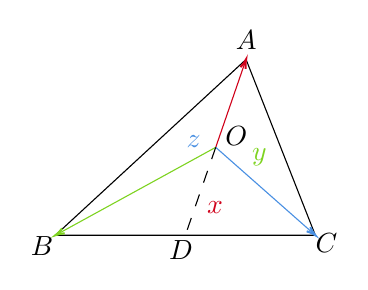
\begin{tikzpicture}[x=0.75pt,y=0.75pt,yscale=-1,xscale=1]
            %uncomment if require: \path (0,300); %set diagram left start at 0, and has height of 300

            %Shape: Triangle [id:dp41718545377725946] 
            \draw   (375.51,83.71) -- (408.89,168.41) -- (283.68,168.41) -- cycle ;
            %Straight Lines [id:da7430270455389383] 
            \draw [color={rgb, 255:red, 208; green, 2; blue, 27 }  ,draw opacity=1 ]   (360.9,126.06) -- (374.86,85.6) ;
            \draw [shift={(375.51,83.71)}, rotate = 109.04] [color={rgb, 255:red, 208; green, 2; blue, 27 }  ,draw opacity=1 ][line width=0.75]    (4.37,-1.32) .. controls (2.78,-0.56) and (1.32,-0.12) .. (0,0) .. controls (1.32,0.12) and (2.78,0.56) .. (4.37,1.32)   ;
            %Straight Lines [id:da21281938084173158] 
            \draw [color={rgb, 255:red, 126; green, 211; blue, 33 }  ,draw opacity=1 ]   (360.9,126.06) -- (285.43,167.45) ;
            \draw [shift={(283.68,168.41)}, rotate = 331.26] [color={rgb, 255:red, 126; green, 211; blue, 33 }  ,draw opacity=1 ][line width=0.75]    (4.37,-1.32) .. controls (2.78,-0.56) and (1.32,-0.12) .. (0,0) .. controls (1.32,0.12) and (2.78,0.56) .. (4.37,1.32)   ;
            %Straight Lines [id:da9898483314704938] 
            \draw [color={rgb, 255:red, 74; green, 144; blue, 226 }  ,draw opacity=1 ]   (360.9,126.06) -- (407.4,167.09) ;
            \draw [shift={(408.89,168.41)}, rotate = 221.42] [color={rgb, 255:red, 74; green, 144; blue, 226 }  ,draw opacity=1 ][line width=0.75]    (4.37,-1.32) .. controls (2.78,-0.56) and (1.32,-0.12) .. (0,0) .. controls (1.32,0.12) and (2.78,0.56) .. (4.37,1.32)   ;
            %Straight Lines [id:da3636995020748923] 
            \draw  [dash pattern={on 4.5pt off 4.5pt}]  (360.9,126.06) -- (346.2,168.61) ;

            % Text Node
            \draw (369.32,68.68) node [anchor=north west][inner sep=0.75pt]    {$A$};
            % Text Node
            \draw (270.57,167.59) node [anchor=north west][inner sep=0.75pt]    {$B$};
            % Text Node
            \draw (407.73,166.45) node [anchor=north west][inner sep=0.75pt]    {$C$};
            % Text Node
            \draw (337.18,169.95) node [anchor=north west][inner sep=0.75pt]    {$D$};
            % Text Node
            \draw (364.32,114.58) node [anchor=north west][inner sep=0.75pt]    {$O$};
            % Text Node
            \draw (355.55,150.73) node [anchor=north west][inner sep=0.75pt]  [color={rgb, 255:red, 208; green, 2; blue, 27 }  ,opacity=1 ]  {$x$};
            % Text Node
            \draw (377.2,125.64) node [anchor=north west][inner sep=0.75pt]  [color={rgb, 255:red, 126; green, 211; blue, 33 }  ,opacity=1 ]  {$y$};
            % Text Node
            \draw (345.63,119.18) node [anchor=north west][inner sep=0.75pt]  [color={rgb, 255:red, 74; green, 144; blue, 226 }  ,opacity=1 ]  {$z$};


        \end{tikzpicture}
    \end{center}
\end{lemma}

\begin{proof}
    延长 $AO$ 交 $BC$ 于点 $D$,

    则$\frac{\mathrm{S}_{\triangle OAB}+\mathrm{S}_{\triangle OAC}}{\mathrm{S}_{\triangle OBC}}=\frac{y+z}{x}=\frac{AO}{OD}$,

    $\therefore x \lvec{OA}=-(y+z) \lvec{OD}$,

    从而$x \lvec{OA}+(y+z) \lvec{OD}=\boldsymbol{0}$. (1)

    又由 $\frac{\mathrm{S}_{\triangle OAB}}{\mathrm{S}_{\triangle OAC}}=\frac{z}{y}=\frac{BD}{CD}$,

    $\therefore y \lvec{BD}=z \lvec{DC}$,

    即 $y(\lvec{OD}-\lvec{OB})=z(\lvec{OC}-\lvec{OD})$,

    $\therefore \lvec{OD}=\frac{y}{y+z} \lvec{OB}+\frac{z}{y+z} \lvec{OC}$,

    代入(1)式得: $x \lvec{OA}+y \lvec{OB}+z \lvec{OC}=\boldsymbol{0}$.
\end{proof}


\subsection{重心的向量表达}
\begin{proposition}
    对于 $\triangle ABC$, 若 $\lvec{GA}+\lvec{GB}+\lvec{GC}=\boldsymbol{0}$, 则 $G$ 是 $\triangle ABC$ 的重心;反之亦成立.
\end{proposition}

\begin{proposition}
    $G$ 是 $\triangle ABC$ 的重心, $P$ 是 $\triangle ABC$ 所在平面上任一点, 则 $\lvec{PG}=\frac{1}{3}(\lvec{PA}+\lvec{PB}+\lvec{PC})$;反之亦成立.
\end{proposition}

\begin{proposition}
    已知 $O$ 是平面上一定点, $A, B, C$ 是平面上不共线的三点, 动点 $P$ 满足 $\lvec{OP}=\lvec{OA}+\lambda(\lvec{AB}+\lvec{AC}), \lambda \in(0,+\infty)$, 则 $P$ 的轨迹一定通过 $\triangle ABC$ 的重心.
\end{proposition}

\subsection{垂心的向量表达}
\begin{proposition}
    对于 $\triangle ABC$, 若 $\tan A \cdot \lvec{HA}+\tan B \cdot \lvec{HB}+\tan C \cdot \lvec{HC}=\boldsymbol{0}$, 则 $H$ 是 $\triangle ABC$ 的垂心;反之亦成立.
\end{proposition}

\begin{proposition}
    $H$ 是 $\triangle ABC$ 所在平面上一点, 若 $\lvec{HA} \cdot \lvec{HB}=\lvec{HB} \cdot \lvec{HC}=\lvec{HC} \cdot \lvec{HA}$, 则 $H$ 是 $\triangle ABC$ 的垂心;反之亦成立.
\end{proposition}

\begin{proposition}
    已知 $O$ 是平面上一定点, $A, B, C$ 是平面上不共线的三点, 动点 $P$ 满足
    $\lvec{OP}=\lvec{OA}+\lambda\left(\frac{\lvec{AB}}{|\lvec{AB}| \cos B}+\frac{\lvec{AC}}{|\lvec{AC}| \cos C}\right), \lambda \in(0,+\infty)$, 则 $P$ 的轨迹一定通过 $\triangle ABC$ 的垂心.
\end{proposition}

\begin{proof}
    由题意得 $\lvec{AP}=\lambda\left(\frac{\lvec{AB}}{|\lvec{AB}| \cos B}+\frac{\lvec{AC}}{|\lvec{AC}| \cos C}\right)$

    \begin{align*}
        \begin{aligned}
             & \text { 而 }\left(\frac{\lvec{AB}}{|\lvec{AB}| \cos B}+\frac{\lvec{AC}}{|\lvec{AC}| \cos C}\right) \cdot \lvec{BC}=\frac{\lvec{AB} \cdot \lvec{BC}}{|\lvec{AB}| \cos B}+\frac{\lvec{AC} \cdot \lvec{BC}}{|\lvec{AC}| \cos C} \\
             & =-|\lvec{BC}|+|\lvec{BC}|                                                                                                                                                                                                   \\
             & =0
        \end{aligned}
    \end{align*}

    $\therefore \lvec{AP} \perp \lvec{BC}$, 动点 $P$ 的轨迹一定通过 $\triangle ABC$ 的垂心.
\end{proof}

\subsection{内心的向量表达}
\begin{proposition}
    对于 $\triangle ABC$, 设 $\mathrm{AB}=c, \mathrm{AC}=b, \mathrm{BC}=a$, 若 $a \cdot \lvec{IA}+b \cdot \lvec{IB}+c \cdot \lvec{IC}=\boldsymbol{0}$, 则点 $I$ 是 $\triangle ABC$ 的内心;反之亦成立.
\end{proposition}

\begin{proof}
    $\because \lvec{IB}=\lvec{IA}+\lvec{AB}, \lvec{IC}=\lvec{IA}+\lvec{AC}$, 代入 $a \cdot \lvec{IA}+b \cdot \lvec{IB}+c \cdot \lvec{IC}=\boldsymbol{0}$ 得\\
    $(a+b+c) \cdot \lvec{IA}+b \cdot \lvec{AB}+c \cdot \lvec{AC}=\boldsymbol{0}$,\\
    $\because b \cdot \lvec{AB}+c \cdot \lvec{AC}=|\lvec{AC}| \cdot \lvec{AB}+|\lvec{AB}| \cdot \lvec{AC}$\\
    $=|\lvec{AB}| \cdot|\lvec{AC}| \cdot\left(\frac{\lvec{AB}}{|\lvec{AB}|}+\frac{\lvec{AC}}{|\lvec{AC}|}\right)$\\
    $=bc\left(\frac{\lvec{AB}}{|\lvec{AB}|}+\frac{\lvec{AC}}{|\lvec{AC}|}\right)$\\
    $\therefore \lvec{AI}=\frac{bc}{a+b+c}\left(\frac{\lvec{AB}}{|\lvec{AB}|}+\frac{\lvec{AC}}{|\lvec{AC}|}\right)$\\
    $\therefore AI$ 与 $\angle BAC$ 的角平分线共线, 即 $AI$ 平分 $\angle BAC$\\
    同理 $BI$ 平分 $\angle ABC, CI$ 平分 $\angle ACB$, 从而 $I$ 是 $\triangle ABC$ 的内心.
\end{proof}

\begin{proposition}
    对于 $\triangle ABC$, 若 $O$ 满足

    $$
        \lvec{OA} \cdot\left(\frac{\lvec{AB}}{|\lvec{AB}|}-\frac{\lvec{AC}}{|\lvec{AC}|}\right)=\lvec{OB} \cdot\left(\frac{\lvec{BA}}{|\lvec{BA}|}-\frac{\lvec{BC}}{|\lvec{BC}|}\right)=\lvec{OC} \cdot\left(\frac{\lvec{CA}}{|\lvec{CA}|}-\frac{\lvec{CB}}{|\lvec{CB}|}\right)=0,
    $$
    则点 $O$ 是 $\triangle ABC$ 的内心;反之亦成立.
\end{proposition}

\subsection{外心的向量表达}
\begin{proposition}
    对于 $\triangle ABC$, 若 $\sin 2A \cdot \lvec{OA}+\sin 2B \cdot \lvec{OB}+\sin 2C \cdot \lvec{OC}=\boldsymbol{0}$, 则 $O$ 是 $\triangle ABC$ 的外心;反之亦成立.
\end{proposition}

\begin{proposition}
    $O$ 是 $\triangle ABC$ 所在平面上一点, 若 $\lvec{OA}^{2}=\lvec{OB}^{2}=\lvec{OC}^{2}$, 则 $O$ 是 $\triangle ABC$ 的外心;反之亦成立.
\end{proposition}

\begin{proposition}
    已知 $O$ 是平面上一定点, $A, B, C$ 是平面上不共线的三点, 动点 $P$ 满足 $\lvec{OP}=\frac{\lvec{OB}+\lvec{OC}}{2}+\lambda\left(\frac{\lvec{AB}}{|\lvec{AB}| \cos B}+\frac{\lvec{AC}}{|\lvec{AC}| \cos C}\right), \lambda \in(0,+\infty)$, 则 $P$ 的轨迹一定通过 $\triangle ABC$ 的外心.
\end{proposition}

\begin{proof}
    设边 $BC$ 的中点为 $M$, 则 $\lvec{OM}=\frac{\lvec{OB}+\lvec{OC}}{2}$, 由题意得
    $$
        \lvec{MP}=\lambda\left(\frac{\lvec{AB}}{|\lvec{AB}| \cos B}+\frac{\lvec{AC}}{|\lvec{AC}| \cos C}\right)
    $$

    \begin{align*}
        \text { 而 }
        \left(\frac{\lvec{AB}}{|\lvec{AB}| \cos B}+\frac{\lvec{AC}}{|\lvec{AC}| \cos C}\right) \cdot \lvec{BC} & =\frac{\lvec{AB} \cdot \lvec{BC}}{|\lvec{AB}| \cos B}+\frac{\lvec{AC} \cdot \lvec{BC}}{|\lvec{AC}| \cos C} \\
                                                                                                               & =-|\lvec{BC}|+|\lvec{BC}|                                                                                  \\
                                                                                                               & =0
    \end{align*}

    $\therefore \lvec{AM} \perp \lvec{BC}, P$ 的轨迹一定通过 $\triangle ABC$ 的外心.
\end{proof}

\subsection{欧拉定理的向量表达}
\begin{proposition}
    若 $O, H$ 分别是 $\triangle ABC$ 的外心和垂心, 则 $\lvec{OH}=\lvec{OA}+\lvec{OB}+\lvec{OC}$.
\end{proposition}

\begin{proof}
    连接 $BO$ 延长交圆 $O$ 于点 $D$, 连接 $AD, CD$, 则 $AD \perp AB, BC \perp CD$\\
    又 $CH \perp AB, AH \perp BC$\\
    $\therefore CH \parallel AD, AH \parallel CD$\\
    $\therefore$ 四边形 $ADCH$ 为平行四边形\\
    $\therefore \lvec{AH}=\lvec{DC}=\lvec{DO}+\lvec{OC}=\lvec{OB}+\lvec{OC}$\\
    $\therefore \lvec{OH}=\lvec{OA}+\lvec{AH}=\lvec{OA}+\lvec{OB}+\lvec{OC}$.
\end{proof}

\tikzset{every picture/.style={line width=0.75pt}} %set default line width to 0.75pt        

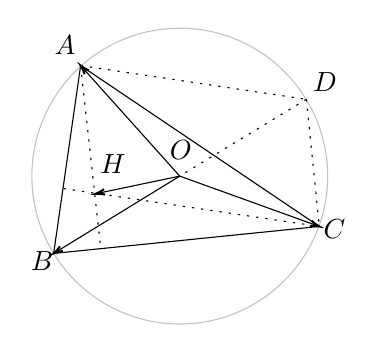
\begin{tikzpicture}[x=0.75pt,y=0.75pt,yscale=-1,xscale=1]
    %uncomment if require: \path (0,300); %set diagram left start at 0, and has height of 300

    %Shape: Circle [id:dp8638038572746185] 
    \draw  [color={rgb, 255:red, 196; green, 193; blue, 193 }  ,draw opacity=1 ] (276.75,155.75) .. controls (276.75,116.4) and (308.65,84.5) .. (348,84.5) .. controls (387.35,84.5) and (419.25,116.4) .. (419.25,155.75) .. controls (419.25,195.1) and (387.35,227) .. (348,227) .. controls (308.65,227) and (276.75,195.1) .. (276.75,155.75) -- cycle ;
    %Straight Lines [id:da5117781865796789] 
    \draw    (300.25,102.5) -- (287.25,193) ;
    %Straight Lines [id:da40133194140523853] 
    \draw    (300.25,102.5) -- (415.25,180) ;
    %Straight Lines [id:da9190277466348651] 
    \draw    (287.25,193) -- (415.25,180) ;
    %Straight Lines [id:da030337826743070506] 
    \draw  [dash pattern={on 0.84pt off 2.51pt}]  (300.25,102.5) -- (310,191.25) ;
    %Straight Lines [id:da6462402259947018] 
    \draw  [dash pattern={on 0.84pt off 2.51pt}]  (292,161.75) -- (415.25,180) ;
    %Straight Lines [id:da6722741273531898] 
    \draw    (348,155.75) -- (288.96,191.95) ;
    \draw [shift={(287.25,193)}, rotate = 328.48] [color={rgb, 255:red, 0; green, 0; blue, 0 }  ][line width=0.75]    (4.37,-1.32) .. controls (2.78,-0.56) and (1.32,-0.12) .. (0,0) .. controls (1.32,0.12) and (2.78,0.56) .. (4.37,1.32)   ;
    %Straight Lines [id:da48269426050329733] 
    \draw    (348,155.75) -- (301.59,103.99) ;
    \draw [shift={(300.25,102.5)}, rotate = 48.12] [color={rgb, 255:red, 0; green, 0; blue, 0 }  ][line width=0.75]    (4.37,-1.32) .. controls (2.78,-0.56) and (1.32,-0.12) .. (0,0) .. controls (1.32,0.12) and (2.78,0.56) .. (4.37,1.32)   ;
    %Straight Lines [id:da4597963546280104] 
    \draw    (348,155.75) -- (413.37,179.32) ;
    \draw [shift={(415.25,180)}, rotate = 199.83] [color={rgb, 255:red, 0; green, 0; blue, 0 }  ][line width=0.75]    (4.37,-1.32) .. controls (2.78,-0.56) and (1.32,-0.12) .. (0,0) .. controls (1.32,0.12) and (2.78,0.56) .. (4.37,1.32)   ;
    %Straight Lines [id:da19024306376007294] 
    \draw [color={rgb, 255:red, 0; green, 0; blue, 0 }  ,draw opacity=1 ]   (348,155.75) -- (309.46,163.84) ;
    \draw [shift={(307.5,164.25)}, rotate = 348.15] [color={rgb, 255:red, 0; green, 0; blue, 0 }  ,draw opacity=1 ][line width=0.75]    (4.37,-1.32) .. controls (2.78,-0.56) and (1.32,-0.12) .. (0,0) .. controls (1.32,0.12) and (2.78,0.56) .. (4.37,1.32)   ;
    %Straight Lines [id:da30127359953371946] 
    \draw  [dash pattern={on 0.84pt off 2.51pt}]  (300.25,102.5) -- (409,118.75) ;
    %Straight Lines [id:da8720800419583445] 
    \draw  [dash pattern={on 0.84pt off 2.51pt}]  (409,118.75) -- (415.25,180) ;
    %Straight Lines [id:da023165060311018726] 
    \draw  [dash pattern={on 0.84pt off 2.51pt}]  (409,118.75) -- (348,155.75) ;

    % Text Node
    \draw (286.5,86.9) node [anchor=north west][inner sep=0.75pt]    {$A$};
    % Text Node
    \draw (275,190.9) node [anchor=north west][inner sep=0.75pt]    {$B$};
    % Text Node
    \draw (416,175.4) node [anchor=north west][inner sep=0.75pt]    {$C$};
    % Text Node
    \draw (411,104.4) node [anchor=north west][inner sep=0.75pt]    {$D$};
    % Text Node
    \draw (342,137.4) node [anchor=north west][inner sep=0.75pt]    {$O$};
    % Text Node
    \draw (308.5,143.9) node [anchor=north west][inner sep=0.75pt]    {$H$};


\end{tikzpicture}
\hspace{2cm}
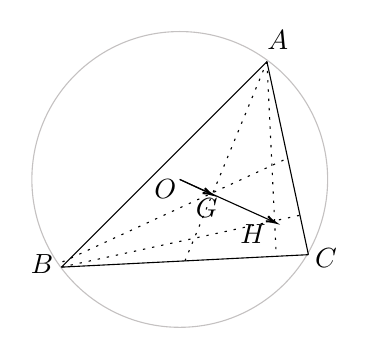
\begin{tikzpicture}[x=0.75pt,y=0.75pt,yscale=-1,xscale=1]
    %uncomment if require: \path (0,300); %set diagram left start at 0, and has height of 300

    %Shape: Circle [id:dp5576661954222375] 
    \draw  [color={rgb, 255:red, 196; green, 193; blue, 193 }  ,draw opacity=1 ] (276.75,155.75) .. controls (276.75,116.4) and (308.65,84.5) .. (348,84.5) .. controls (387.35,84.5) and (419.25,116.4) .. (419.25,155.75) .. controls (419.25,195.1) and (387.35,227) .. (348,227) .. controls (308.65,227) and (276.75,195.1) .. (276.75,155.75) -- cycle ;
    %Straight Lines [id:da7258859971367271] 
    \draw    (390,99) -- (291,198) ;
    %Straight Lines [id:da3156736380760452] 
    \draw    (390,99) -- (410,192) ;
    %Straight Lines [id:da7465470237686334] 
    \draw    (291,198) -- (410,192) ;
    %Straight Lines [id:da033955443365715654] 
    \draw  [dash pattern={on 0.84pt off 2.51pt}]  (291,198) -- (406,173) ;
    %Straight Lines [id:da7312470733297733] 
    \draw  [dash pattern={on 0.84pt off 2.51pt}]  (291.5,195.5) -- (400,145.5) ;
    %Straight Lines [id:da9722534008421468] 
    \draw    (348,155.75) -- (361.69,162.15) ;
    \draw [shift={(363.5,163)}, rotate = 205.07] [color={rgb, 255:red, 0; green, 0; blue, 0 }  ][line width=0.75]    (4.37,-1.32) .. controls (2.78,-0.56) and (1.32,-0.12) .. (0,0) .. controls (1.32,0.12) and (2.78,0.56) .. (4.37,1.32)   ;
    %Straight Lines [id:da5490453987009081] 
    \draw    (348,155.75) -- (392.18,175.68) ;
    \draw [shift={(394,176.5)}, rotate = 204.28] [color={rgb, 255:red, 0; green, 0; blue, 0 }  ][line width=0.75]    (4.37,-1.32) .. controls (2.78,-0.56) and (1.32,-0.12) .. (0,0) .. controls (1.32,0.12) and (2.78,0.56) .. (4.37,1.32)   ;
    %Straight Lines [id:da9976698491167126] 
    \draw  [dash pattern={on 0.84pt off 2.51pt}]  (390,99) -- (394.5,192.5) ;
    %Straight Lines [id:da4368693118593838] 
    \draw  [dash pattern={on 0.84pt off 2.51pt}]  (350.5,195) -- (390,99) ;

    % Text Node
    \draw (389,82.9) node [anchor=north west][inner sep=0.75pt]    {$A$};
    % Text Node
    \draw (275,190.9) node [anchor=north west][inner sep=0.75pt]    {$B$};
    % Text Node
    \draw (412,187.9) node [anchor=north west][inner sep=0.75pt]    {$C$};
    % Text Node
    \draw (354.5,163.9) node [anchor=north west][inner sep=0.75pt]    {$G$};
    % Text Node
    \draw (334.5,154.4) node [anchor=north west][inner sep=0.75pt]    {$O$};
    % Text Node
    \draw (376,176.4) node [anchor=north west][inner sep=0.75pt]    {$H$};


\end{tikzpicture}

\begin{proposition}
    若 $O, G, H$ 分别是 $\triangle ABC$ 的外心, 重心, 垂心, 则 $\lvec{OG}=\frac{1}{3} \lvec{OH}$.
\end{proposition}

\begin{proof}
    $\because G$ 是重心, 由命题 2 知 $\lvec{OG}=\frac{1}{3}(\lvec{OA}+\lvec{OB}+\lvec{OC})$\\
    又由命题 12 知 $\lvec{OH}=\lvec{OA}+\lvec{OB}+\lvec{OC}$\\
    $\therefore \lvec{OG}=\frac{1}{3} \lvec{OH}$.
\end{proof}

\section{练习题}
\begin{exercise}
    已知 $O$ 是 $\triangle ABC$ 的重心, 点 $P$ 满足 $\lvec{OP}=\frac{1}{3}\left(\frac{1}{2} \lvec{OA}+\frac{1}{2} \lvec{OB}+2 \lvec{OC}\right)$, 则点 $P$ 一定是 $\triangle ABC$ 的( \quad ). \\
    A. $AB$ 边中线的中点 \qquad B. $AB$ 边中线的三等分点(非重心) \\
    C. 重心 \qquad D. $AB$ 边的中点
\end{exercise}

\begin{exercise}
    $O$ 是 $\triangle ABC$ 所在平面上一点, 若 $\lvec{OA}^{2}+\lvec{BC}^{2}=\lvec{OB}^{2}+\lvec{CA}^{2}=\lvec{OC}^{2}+\lvec{AB}^{2}$, 则 $O$ 是 $\triangle ABC$ 的( \quad ). \\
    A. 外心 \qquad B. 内心 \qquad C. 垂心 \qquad D. 重心
\end{exercise}

\begin{exercise}
    $P$ 是 $\triangle ABC$ 所在平面上一点, 若 $\lvec{PA} \cdot \lvec{PB}+\lvec{PB} \cdot \lvec{PC}+\lvec{PA} \cdot \lvec{PC}=0$, 则 $P$ 是 $\triangle ABC$ 的( \quad ). \\
    A. 外心 \qquad B. 内心 \qquad C. 垂心 \qquad D. 重心
\end{exercise}

\begin{exercise}
    $P$ 是 $\triangle ABC$ 所在平面上一点, 若 $\lvec{CA}^{2}=\lvec{CB}^{2}-2 \lvec{AB} \cdot \lvec{CP}$, 则 $P$ 的轨迹一定通过 $\triangle ABC$ 的( \quad ). \\
    A. 外心 \qquad B. 内心 \qquad C. 垂心 \qquad D. 重心
\end{exercise}

\begin{exercise}
    已知非零向量 $\lvec{AB}, ~ \lvec{AC}$ 满足 $\left(\frac{\lvec{AB}}{|\lvec{AB}|}+\frac{\lvec{AC}}{|\lvec{AC}|}\right) \cdot \lvec{BC}=0$, 且 $\frac{\lvec{AB}}{|\lvec{AB}|} \cdot \frac{\lvec{AC}}{|\lvec{AC}|}=\frac{1}{2}$, 则 $\triangle ABC$ 为( \quad ). \\
    A. 三边均不相等的三角 \qquad B. 直角三角形 \\
    C. 等腰非等边三角形 \qquad D. 等边三角形
\end{exercise}

\begin{exercise}
    $P$ 是 $\triangle ABC$ 所在平面内与 $A$ 不重合的一点, 且满足 $\lvec{AB}+\lvec{AC}=3 \lvec{AP}$, 则 $P$ 是 $\triangle ABC$ 的( \quad ). \\
    A. 外心 \qquad B. 内心 \qquad C. 垂心 \qquad D. 重心
\end{exercise}

\begin{exercise}
    已知 $O$ 是 $\triangle ABC$ 的外接圆的圆心, 半径为 1, 且 $\lvec{OA}+\lvec{OB}+\lvec{OC}=\boldsymbol{0}$, 则 $\lvec{OA} \cdot \lvec{OB}$ 等于 ( \quad ).
\end{exercise}

\begin{exercise}
    $\triangle ABC$ 的外接圆圆心为 $O$, 两条边上的高的交点为 $H$, 若 $\lvec{OH}=m(\lvec{OA}+\lvec{OB}+\lvec{OC})$, 则实数 $m=$ ( \quad ).
\end{exercise}

\begin{exercise}
    已知 $G$ 是 $\triangle ABC$ 的重心, 过 $G$ 作直线与 $AB, AC$ 分别相交于 $M, N$ 两点, 若 $\lvec{AM}=x \lvec{AB}, \lvec{AN}=y \lvec{AC}$, 则 $\frac{1}{x}+\frac{1}{y}=$ ( \quad ).
\end{exercise}

\texttt{答案: 1-6 BCCADD \quad 7. -1/2 \quad  8. 1  \quad 9. 3}
%\chapter{复数}

%\chapter{立体几何初步}
%\section{基本立体图形}
%\section{立体图形的直观图I}
%\section{立体图形的直观图II}
%\section{棱柱、棱锥、棱台的表面积与体积}
%\section{圆柱、圆锥、圆台的表面积与体积}
\section{球的表面积与体积}
\marginnote{2024-4-29}
\subsection{球的表面积}
我们在初中都学过圆的面积, 设圆的半径为 $r$, 则圆的面积为
 $$
 S = \uppi r^{2}. 
 $$ 
 上式说明圆的面积和半径有关, 进一步地讲, 圆的面积作为二维平面上的度量, 它和圆的半径的平方成正比. 此外, 圆的面积还包含了常数 $\uppi$. 类似地, 同样是求面积, 我们是否可以推测球的表面积也和球的半径平方成正比呢?是否也和常数 $\uppi$ 有关呢?
\begin{formula}[球的表面积]
	设球的半径为 $r$, 则球的表面积
	$$
		S_{\text{球}}= 4 \uppi r^{2}.
	$$
\end{formula}
下面给出一个不太严谨的球的表面积公式的证明方法, 主要是利用圆柱侧面积来近似代替球的表面积. 
\begin{proof}
  把一个半径为 $r$ 的球的上半球横向切成 $n$ (无穷大)份, 每份等高并且把每份看成一个类似圆柱, 其中半径等于底面圆半径, 则从下到上第 $k$ 个圆柱的侧面积为
  $$
  S(k)=2 \uppi r_k h .
  $$
  $$
  \begin{aligned}
  & \because h=\frac{r}{n}, r_k=\sqrt{r^2-(k h)^2}, \\
  & \therefore S(k)=\frac{2 \uppi r}{n} \sqrt{r^2-(k h)^2}=2 \uppi r^2 \sqrt{\frac{1}{n^2}-\frac{k^2}{n^4}} . \\
  & \therefore S_{\text {球 }}=\lim _{n \rightarrow+\infty} 2[S(1)+S(2)+\cdots+S(n)]=4 \uppi r^2 .
  \end{aligned}
  $$
\end{proof}  

\begin{formula}[球的体积]
	设球的半径为 $r$, 则球的体积
  $$
  V_{\text{球}}=\frac{4}{3} \uppi r^{3}.
  $$
\end{formula}

\begin{example}
	如图 8.3-4, 某种浮标由两个半球和一个圆柱黏合而成,半球的直径是 $0.3 \mathrm{~m}$, 圆柱高 $0.6 \mathrm{~m}$. 如果在浮标表面涂一层防水漆, 每平方米需要 $0.5 \mathrm{~kg}$ 涂料, 那么给 1000 个这样的浮标涂防水漆需要多少涂料? ( $\uppi$ 取 3.14)
\end{example}
\begin{solution}
一个浮标的表面积为
	$$
		2 \uppi \times 0.15 \times 0.6+4 \uppi \times 0.15^2=0.8478\left(\mathrm{~m}^2\right),
	$$

	所以给 1000 个这样的浮标涂防水漆约需涂料
	$$
		0.8478 \times 0.5 \times 1000=423.9(\mathrm{~kg}) .
	$$
\end{solution}


类比利用圆周长求圆面积的方法, 我们可以利用球的表面积求球的体积. 如图8.3-5,把球 $O$ 的表面分成 $n$ 个小网格, 连接球心 $O$ 和每个小网格的顶点, 整个球体就被分割成 $n$ 个 “小锥体”.

当 $n$ 越大, 每个小网格越小时, 每个 “小锥体” 的底面就越平, “小锥体” 就越近似于棱雉, 其高越近似于球半径 $R$. 设 $O-A B C D$ 是其中一个 “小锥体”, 它的体积
$$
V_{O-A B C D} \approx \frac{1}{3} S_{A B C D} R . 
$$

由于球的体积就是这 $n$ 个 “小锥体” 的体积之和, 而这 $n$ 个 “小锥体” 的底面积之和就是球的表面积. 因此, 球的体积
$$
V_{\text {球 }}=\frac{1}{3} S_{\text {球 }} R=\frac{1}{3} \times 4 \uppi R^2 \cdot R=\frac{4}{3} \uppi R^3 . 
$$

由此, 我们得到球的体积公式
$$
V_{\text {球 }}=\frac{4}{3} \uppi R^3 .
$$

\bibliography{refs} % 设置参考文献文件为references.bib
\end{document}